%% Tex spellcheck
% Maybe put this as Chapter 2

% Write in English.
\chapter{Chapter 1 :  State of the art}

Some companies are already selling fully configurable \gls{gnss} simulators with included software and support for every \gls{gnss} technologies. These simulators are very expensive and are not open source, thus hardly customizable. They also are massive and difficult to transport and usually require a dedicated computer with a specific software to control them.


\section{Spirent}

Spirent is a company that sells \gls{gnss} simulators. They offer a wide range of products from single-frequency to multi-frequency simulators. They also offer a wide range of software to configure and control the simulators. The software is user-friendly and offers a wide range of features. The simulators are very expensive and are not open source.

Here's an example of a Spirent simulator:
\begin{figure}[H]
    \centering
    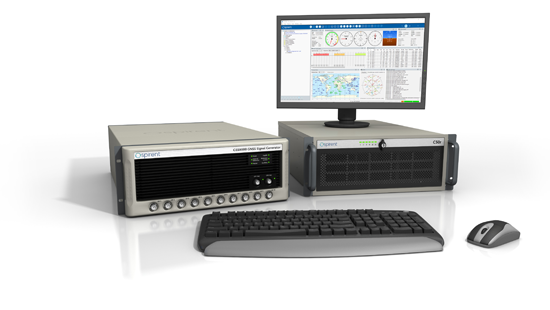
\includegraphics[width=1\linewidth]{gss9000gui.png}
    \caption[Spirent GSS9000 gnss simulator]{Spirent GSS9000 gnss simulator Source: www.e-education.psu.edu ref: URL14}
    \label{fig:spirent_gss9000gui}
\end{figure}


Here's an idea of the software that comes with the simulator:
\begin{figure}[H]
    \centering
    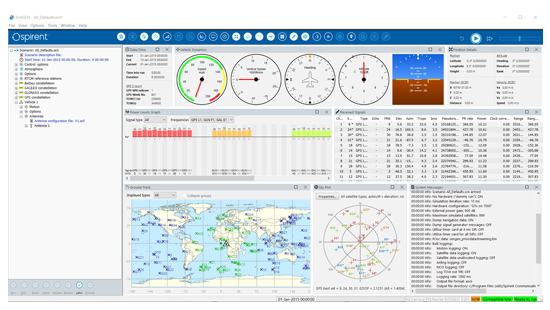
\includegraphics[width=1\linewidth]{spirent_gui.png}
    \caption[Spirent existing software]{Spirent existing software Source: www.e-education.psu.edu ref: URL14}
    \label{fig:spirent_gui}
\end{figure}


\section{Rohde n Schwarz}

Rohde n Schwarz is another company that sells \gls{gnss} simulators. They offer a wide range of products from single-frequency to multi-frequency simulators too. Their devices come at around 50'000 \$ for a base model ...

Here's an example of a Rohde \& Schwarz simulator:

\begin{figure}[H]
    \centering
    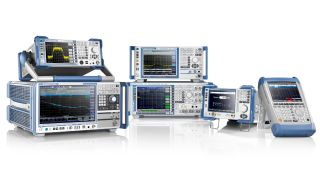
\includegraphics[width=1\linewidth]{rhode.jpg}
    \caption[Rohde n Schwarz]{Rohde n Schwarz Source: www.e-education.psu.edu ref: URL14}
    \label{fig:rhode}
\end{figure}